\chapter{Il PROLOG}

\dfn{PROLOG}{
  PROLOG (Programming Logic) è un \newfancyglitter{linguaggio dichiarativo} basato sul \newfancyglitter{paradigma logico}: 
  \begin{itemize}
    \item Non si descrive cosa fare per risolvere un problema. 
    \item Si descrive la situazione reale con \newfancyglitter{fatti} e \newfancyglitter{regole} e si chiede all'interprete di verificare se un \newfancyglitter{goal} segue oppure no secondo una logica classica.
  \end{itemize}
}

\nt{Il PROLOG è equivalente alla logica dei predicati del primordine.}

\section{Le Basi}

\dfn{Fatti}{Si rappresenta con dei \newfancyglitter{fatti} un dominio di interesse.}

\ex{Fatto}{
  Fatto per descrivere che un alimento contiene più calorie di un altro: 
  \begin{itemize}
    \item piuCalorico(wurstel, banana). 
    \item Rappresenta il fatto che il würstel è un alimento maggiormente
calorico rispetto alla banana.
  \end{itemize}
}

\dfn{Regole}{
  Si rappresentano le possibili inferenze con delle \newfancyglitter{regole}: 
  \begin{center}
    \texttt{head := subgoal1, subgoal2, \dots, subgoaln}
  \end{center}
}

\ex{Regola}{
  \begin{center}
    \texttt{felino(X) := gatto(X)}
  \end{center}
  Rappresenta la regola che permette di concludere che i gatti sono felini.
}

\paragraph{Idee di base del PROLOG:}

\begin{itemize}
  \item Regole ricorsive.
  \item L'interprete analizza i fatti e le regole nell'ordine in cui si trovano nel programma. 
  \item Meccanismo di pattern matching per uni care
variabili e termini. 
\item L’interprete, dato un programma, cerca di
dimostrare un goal considerando fatti e applicando
regole, nel secondo caso generando sotto-goal.
\end{itemize}

\dfn{Clausole}{
  Le clausole sono i fatti o le regole. Contengono:
  \begin{itemize}
    \item Atomi: 
      \begin{itemize}
        \item Costanti. 
        \item Numeri.
      \end{itemize}
    \item Variabili.
    \item Termini Composti, ottenuti applicando funtori a termini.

  \end{itemize}
}

\nt{Un programma PROLOG è un insieme di clausole.}

\clm{}{}{
  \begin{itemize}
    \item L'estensione dei file PROLOG è 'pl'.
    \item In PROLOG le variabili hanno l'iniziale maiuscola. 
    \item L'unica struttura dati nativa è la lista.
    \item Per eseguire swi: swipl. 
    \item Per compilare: $[$'nomefile.pl'$]$.
    \item Il comando ';' indica possibili alternative.
    \item Il comando 'trace.' consente un esecuzione passo per passo.
    \item L'ordine è importante perché PROLOG "legge" dall'alto verso il basso.
\end{itemize}
}

\paragraph{Qualche predicato \fancyglitter{built-in}:}

\begin{itemize}
  \item \texttt{var(X)}: indica se \texttt{X} è una variabile. 
\item \texttt{ground(X)}: indica se \texttt{X} è istanziata. 
\item \texttt{atom(X)}: indica se \texttt{X} è atomica. 
\end{itemize}

\subsection{Liste}

\dfn{Lista}{
  La \newfancyglitter{lista} è la struttura dati principale in PROLOG. Una lista è caratterizzata da una testa e da una
coda: 
\begin{itemize}
  \item Testa: primo termine (a sinistra) della lista. 
  \item Coda: la lista dei termini dal secondo (incluso)
in poi.
\end{itemize}
}

\nt{Rappresentata come $[$Head $|$ Tail$]$.}

\begin{figure}[h]
    \centering
    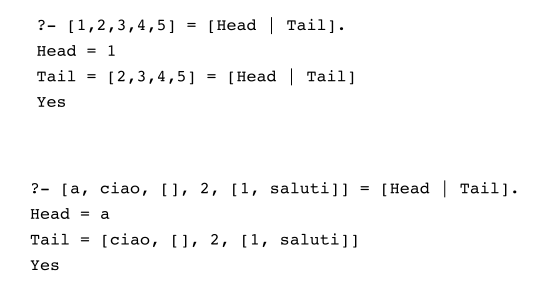
\includegraphics[scale=0.6]{01/liste.png}
    \caption{Le liste in PROLOG.}
\end{figure}

\paragraph{Predicati \fancyglitter{built-in}:}

\begin{itemize}
  \item \texttt{length(Lista, N)}: ha successo se la \texttt{Lista} contiene \texttt{N} elementi. 
  \item \texttt{member(Elemento,Lista)}: ha successo se la \texttt{Lista} contiene il termine \texttt{Elemento}.
  \item \texttt{select(Elemento,Lista,Rimanenti)}: rimuove \texttt{Elemento} da \texttt{Lista} e restituisce \texttt{Rimanenti}. 
\end{itemize}

\section{Interprete PROLOG}

\qs{}{Come avviene l'esecuzione di programmi PROLOG?}

\begin{itemize}
  \item Esecuzione mediante \fancyglitter{backward chaining} in profondità. 
  \item Si parte dal \fancyglitter{goal} che si vuole derivare: 
    \begin{itemize}
      \item \fancyglitter{Goal} = congiunzione di formule atomiche $G_1, G_2, \dots, G_n$. 
      \item Si vuole dimostrare, mediante risoluzione, che il goal segua logicamente dal programma. 
    \end{itemize}
  \item Una regola $A :- B_1, B_2, \dots, B_m$ è applicabile a $G_i$ se: 
    \begin{itemize}
      \item Le variabili vengono rinominate. 
      \item $A$ e $G_i$ unificano. 
    \end{itemize}
\end{itemize}

\begin{figure}[h]
    \centering
    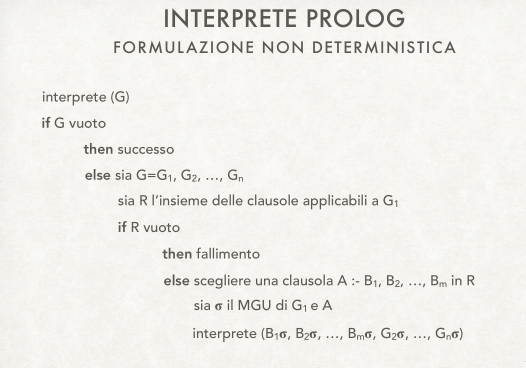
\includegraphics[scale=0.4]{02/Interprete PROLOG.png}
    \caption{Una formulazione non deterministica di come funziona l'interprete PROLOG.}
\end{figure}

\nt{MGU è il Most General Unifier: minimo sforzo per rendere uguali due variabili (il fatto e il goal).}

\begin{itemize}
  \item La computazione ha successo se esiste una computazione che
termina con successo. 
\item Non determinismo: non è specificata la regola scelta in R. 
\item Ma l'interprete PROLOG si comporta in modo \fancyglitter{deterministico}: 
  \begin{itemize}
    \item Le clausole vengono considerate nell’ordine in cui sono scritte
nel programma. 
\item Viene fatto backtracking all’ultimo punto di scelta ogni volta
che la computazione fallisce.
  \end{itemize}
\item In caso di successo, l’interprete restituisce una sostituzione per le
variabili che compaiono nel goal.
\end{itemize}

\subsection{Breve Ripasso di Logica}

\dfn{Logica Classica}{
Conseguenza logica definita semanticamente: dato una teoria e una formula, diciamo che la formula segue dalla
teoria se essa è vera in tutti i modelli della teoria.
}

\ex{Gatti}{
  \begin{itemize}
    \item I gatti miagolano: gatto $\rightarrow$ miagola. 
    \item I persiani sono gatti: persiano $\rightarrow$ gatto.
    \item Si vuole dimostrare che i persiani miagolano: k $\vDash$ persiano $\rightarrow$ miagola.
  \end{itemize} 
  \begin{center}
    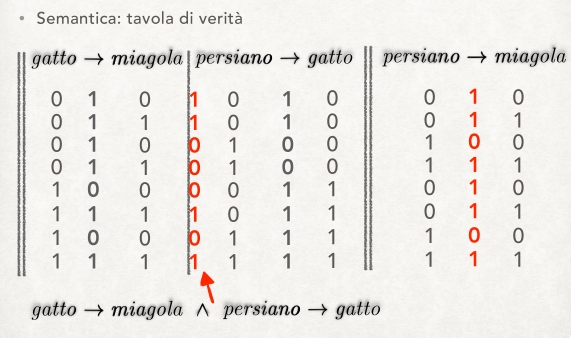
\includegraphics[scale = 0.4]{02/gatto.png}
  \end{center}
}



